Toll payment checkpoints at the toll gates often experience queues and delays as motorists try to pay their toll fees. These queues occur due to issues such as:
\begin{itemize}
    \item Limited manpower to handle the number of vehicles using the station causing congestion especially during moments such as peak hours of morning and evening, but there is limited labour to service them.
    \item Delays as tollgate employees try to find change for motorists since current payment system employs cash payments
\end{itemize}
\begin{figure}
    \begin{center}
        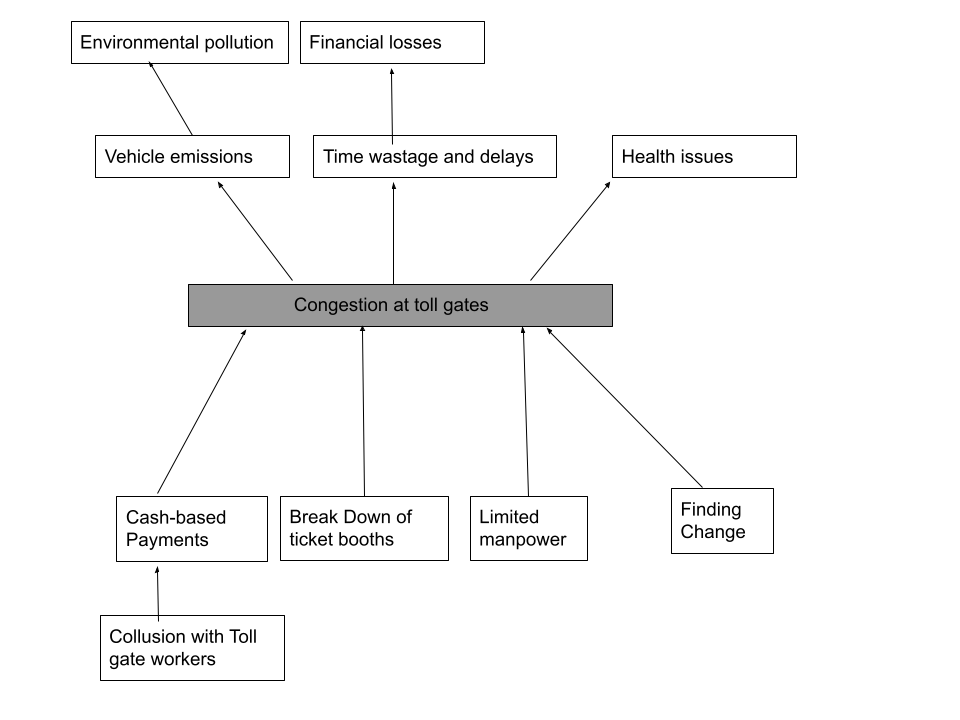
\includegraphics[scale = 0.5]{images/problem}
        \caption{Problem Tree for the research project}
    \end{center}
\end{figure}
Another issue arises when employees managing the systems collude with some motorists who are granted access even without paying the required fees. Implementation of a similar checkpoint system is not limited to tollgates, and is also used in places such as parking ticket systems for public places such as malls, universities\cite{bagadiong_car_2020}, which also suffer similar shortcomings.In this context, there is also an issue of breakdown of the ticketing machines due to low maintenance works

The above issues have their own attached negative effects. One study found that the present state of traffic flow in Uganda, particularly Kampala city causes Uganda losses of approximately 6.7\% of its GDP to traffic congestion annually. Another study by Thomas Munzel found that frequent congestion of vehicles increases the risk of heart failure and other health conditions in motorists.This is caused by the high level of stress during congestion\cite{munzel_environmental_2018}.

From an environmental point of view, the current approach is also unfeasible.This is because the congestion from the delays results in increased carbon emissions from the vehicles, which also puts pedestrians and other road users at risk\cite{zhang_air_2013}. The checkpoint systems used in the parking management context use tickets, assigned to each motorist, which is also not only costly, as a lot of paper is required for printing, yet the paper is needed for a brief time, but it is also a bad practice as trees are cut down to get paper\cite{bajpai_basic_2015}.

The payment approach currently used at these checkpoints is also an issue as these payments are mainly done through physical cash. In light of the recent global CoVID-19 pandemic, there is need to adopt cashless payments leveraging platforms such as mobile money \cite{centellegher_mobile_2018}, as physical cash is known to be a vector for viruses,\cite{angelakis_paper_2014, maritz_filthy_2017} and this would be an opportunity for countries to better future-proof themselves in case of another pandemic or disease outbreak.

Altogether, these factors impede on the establishment of intelligent transportation systems as well as utilisation of techniques like ubiquitous computing for cities like Kampala, and their gradual evolution into smart cities.